\documentclass[aspectratio=169,10pt]{beamer}

\usetheme{default}
\useinnertheme{rectangles}
\setbeamertemplate{navigation symbols}{}
\setbeamersize{text margin left=0.7cm, text margin right=0.7cm}

\usepackage{amsmath,amssymb}
\usepackage[T1]{fontenc}
\usepackage[scaled=0.96]{FiraSans}   % clean humanist sans for all text
\usepackage{newtxsf}                  % matching sans-serif math
\renewcommand{\familydefault}{\sfdefault}
\usepackage{microtype}
\usepackage{booktabs}
\usepackage{graphicx}
\usepackage{animate}
\usepackage{tikz}
\usetikzlibrary{arrows.meta,positioning,calc}

% Slide measures are short: avoid mid-word hyphenation (e.g. "fi-nite").
\hyphenpenalty=10000
\exhyphenpenalty=10000

\definecolor{ink}{HTML}{202121}
\definecolor{forest}{HTML}{0E3B2C}
\definecolor{gold}{HTML}{D8AD62}
\definecolor{gilt}{HTML}{9E7B38}
\definecolor{paper}{HTML}{F4EFE3}
\definecolor{mist}{HTML}{C9CBC7}
\definecolor{muted}{HTML}{60645F}
\definecolor{clay}{HTML}{B04A2F}   % warm accent for the "chaotic" regime / big-step
\definecolor{orderedblue}{HTML}{3A6EA5}

\setbeamercolor{normal text}{fg=ink,bg=paper}
\setbeamercolor{background canvas}{bg=paper}
\setbeamercolor{frametitle}{fg=forest}
\setbeamercolor{structure}{fg=forest}
\setbeamercolor{block title}{fg=white,bg=forest}
\setbeamercolor{block body}{fg=ink,bg=paper!85!mist}
\setbeamercolor{itemize item}{fg=gilt}
\setbeamertemplate{itemize item}{\raisebox{0.15em}{\tiny$\blacktriangleright$}}
\setlength{\abovedisplayskip}{0.4em}
\setlength{\belowdisplayskip}{0.4em}

% Custom frame title: forest text on paper background, gold underline.
\setbeamertemplate{frametitle}{%
  \nointerlineskip
  \vspace{1.05em}
  \begin{beamercolorbox}[wd=\paperwidth,leftskip=0.7cm,rightskip=1.6cm,sep=0pt]{frametitle}%
    {\bfseries\large\insertframetitle}\\[0.12em]
    {\color{gold}\rule{2.6cm}{1.2pt}}%
  \end{beamercolorbox}%
  \vspace{0.2em}
}

\newcommand{\relu}{ReLU}
\newcommand{\E}{\mathbb{E}}
\newcommand{\halfline}{\vspace{0.45em}}
\newcommand{\cmulogo}{assets/logos/Carnegie_Mellon_University_seal.svg-2.png}
\newcommand{\icmllogo}{assets/logos/ICML-logo.png}

% Footer on all (non-plain) slides, with the CMU seal pinned to the top-right.
\setbeamertemplate{footline}{%
  \begin{tikzpicture}[remember picture,overlay]
    \node[anchor=east,opacity=0.52] at ($(current page.north east)+(-0.62,-0.88)$)
      {\includegraphics[height=0.70cm]{\cmulogo}};
    \node[anchor=south west] at ($(current page.south west)+(0.70,0.18)$)
      {\scriptsize\color{muted}Lucas Fernandez-Sarmiento};
    \node[anchor=south] at ($(current page.south)+(0,0.18)$)
      {\scriptsize\color{muted}ICML 2026};
    \node[anchor=south east] at ($(current page.south east)+(-0.70,0.18)$)
      {\scriptsize\color{muted}\insertframenumber};
  \end{tikzpicture}%
  \vbox to 0.36cm{}%
}

\title[Dropout Universality]{Dropout Universality}
\subtitle{Scaling Laws and Optimal Scheduling at the Edge-of-Chaos}
\author{Lucas Fernandez-Sarmiento}
\institute{Carnegie Mellon University}
\date{ICML 2026}

\begin{document}

% -------------------------------------------------------------------------
% Title
% -------------------------------------------------------------------------
\begin{frame}[plain]
  \begin{tikzpicture}[remember picture,overlay]
    \fill[paper] (current page.south west) rectangle (current page.north east);
    \draw[gold,line width=0.8pt]
      ($(current page.north west)+(0.75,-1.95)$) --
      ($(current page.north east)+(-0.75,-1.95)$);
    \node[anchor=north west] at ($(current page.north west)+(0.75,-0.38)$)
      {\includegraphics[height=1.05cm]{\icmllogo}};
    \node[anchor=north east] at ($(current page.north east)+(-0.75,-0.30)$)
      {\includegraphics[height=1.30cm]{\cmulogo}};
  \end{tikzpicture}

  \vspace{2.7cm}
  \begin{center}
    {\color{ink}\bfseries\fontsize{22}{27}\selectfont
    Dropout Universality}\\[0.35em]
    {\color{forest}\fontsize{15}{19}\selectfont
    Scaling Laws and Optimal Scheduling at the Edge-of-Chaos}

    \vspace{0.9cm}
    {\color{gold}\rule{6.0cm}{1.0pt}}

    \vspace{0.7cm}
    {\Large\color{ink} Lucas Fernandez-Sarmiento}\\[0.18em]
    {\large\color{muted} Carnegie Mellon University}

    \vfill
    {\color{muted}ICML 2026}
    \vspace{0.4cm}
  \end{center}
\end{frame}

% -------------------------------------------------------------------------
% Motivation: elephant
% -------------------------------------------------------------------------
\begin{frame}{In search of good variables}
  \begin{columns}[c,onlytextwidth]
    \begin{column}{0.60\textwidth}
      \vspace{0.4em}
      {\color{ink}\itshape\fontsize{11}{14}\selectfont
      ``With four parameters I can fit an elephant, and with five I can make him wiggle his trunk.''}\\[0.35em]
      {\color{gilt}\small von Neumann to Fermi, via Dyson}

      \vspace{1.2em}
      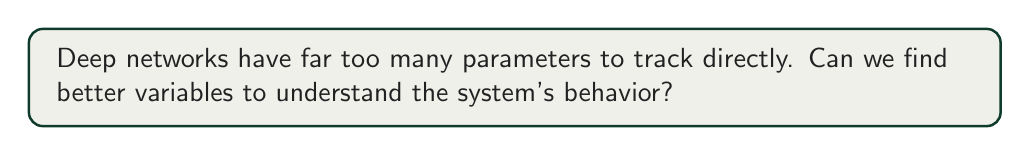
\begin{tikzpicture}
        \node[
          fill=forest!10!paper,
          fill opacity=0.45,
          draw=forest,
          line width=0.9pt,
          text opacity=1,
          text=ink,
          rounded corners=5pt,
          inner xsep=0.35cm,
          inner ysep=0.25cm,
          text width=0.96\linewidth,
          align=left
        ] {Deep networks have far too many parameters to track directly. Can we find better variables to understand the system's behavior? };
      \end{tikzpicture}

    \end{column}

    \begin{column}{0.36\textwidth}
      \centering
      \animategraphics[autoplay,loop,poster=first,width=0.96\linewidth,type=png]%
        {20}{assets/elephant_frames/elephant_}{0}{59}\\[0.35em]
      {\fontsize{4.8}{5.6}\selectfont\color{muted}
      Mayer, Khairy \& Howard\\
      Am.\ J.\ Phys.\ \textbf{78}, 648 (2010)}
    \end{column}
  \end{columns}
\end{frame}

% -------------------------------------------------------------------------
% Mean-field theory
% -------------------------------------------------------------------------
\begin{frame}{Mean Field Theory {\small(Poole et al.)} \& Deep Information Propagation {\small(Schoenholz et al.)}}
  \begin{columns}[T,onlytextwidth]
    \begin{column}{0.36\textwidth}
      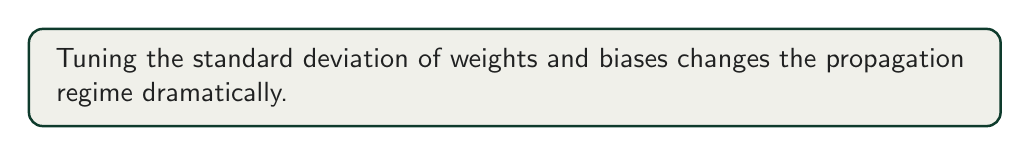
\begin{tikzpicture}
        \node[
          fill=forest!10!paper,
          fill opacity=0.45,
          draw=forest,
          line width=0.9pt,
          text opacity=1,
          text=ink,
          rounded corners=5pt,
          inner xsep=0.35cm,
          inner ysep=0.25cm,
          text width=0.96\linewidth,
          align=left
        ] {Tuning the standard deviation of weights and biases changes the propagation regime dramatically.};
      \end{tikzpicture}
    \end{column}

    \begin{column}{0.60\textwidth}
      \begin{itemize}
        \item {\color{orderedblue}\bfseries Ordered:} signals contract; gradients vanish.
        \item {\color{forest}\bfseries Edge-of-chaos:} information propagates subexponentially.
        \item {\color{clay}\bfseries Chaotic:} signals separate; gradients explode.
      \end{itemize}
    \end{column}
  \end{columns}

  \vspace{-0.55em}
  \begin{center}
    \animategraphics[autoplay,loop,poster=first,height=0.40\textheight,type=png]%
      {16}{assets/manifold_slide_frames_t/manifold_}{0}{200}

    \vspace{-0.05em}
    {\scriptsize\color{muted}A circular input manifold is embedded in high dimension, propagated through random tanh layers, then projected to 2D.}
  \end{center}
\end{frame}

% -------------------------------------------------------------------------
% Correlation length
% -------------------------------------------------------------------------
\begin{frame}{How deep can signals propagate\\ and networks learn?}
  \begin{columns}[T,onlytextwidth]
    \begin{column}{0.40\textwidth}
      \vspace{0.7em}
      Instead of tracking weights, mean-field theory tracks how correlations between inputs change with depth.

      \vspace{1.0em}
      \[
        |c^\ast-c_\ell|
        \;\approx\;
        |c^\ast-c_0|\,e^{-\ell/\xi_c}
      \]

      \vspace{0.8em}
      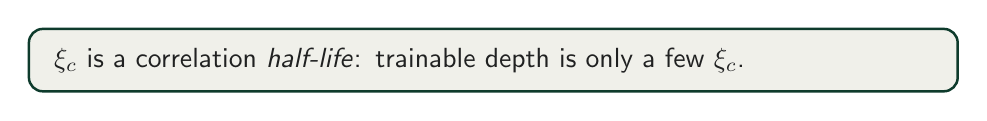
\begin{tikzpicture}
        \node[
          fill=forest!10!paper,
          fill opacity=0.45,
          draw=forest,
          line width=0.9pt,
          text opacity=1,
          text=ink,
          rounded corners=5pt,
          inner xsep=0.32cm,
          inner ysep=0.24cm,
          text width=0.92\linewidth,
          align=left
        ] {\(\xi_c\) is a correlation \emph{half-life}: trainable depth is only a few \(\xi_c\).};
      \end{tikzpicture}
    \end{column}

    \begin{column}{0.56\textwidth}
      \vspace{-1.25em}
      \begin{center}
        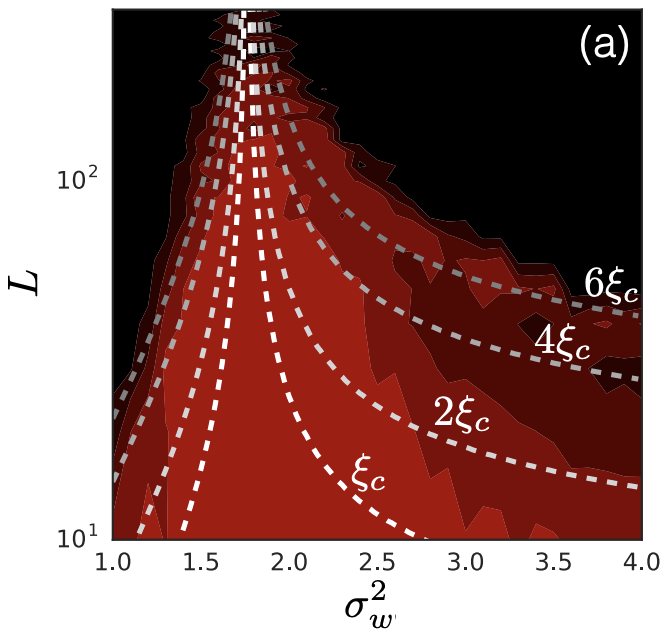
\includegraphics[height=0.66\textheight]{assets/dip_trainability_transparent.png}\\[-0.3em]
        {\tiny\color{muted}Schoenholz et al., \emph{Deep Information Propagation}, ICLR 2017}
      \end{center}
    \end{column}
  \end{columns}
\end{frame}

% -------------------------------------------------------------------------
% Dropout deformation
% -------------------------------------------------------------------------
\begin{frame}{The effect of dropout}
  \vfill
  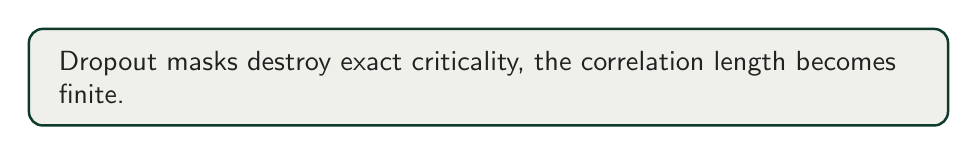
\begin{tikzpicture}
    \node[
      fill=forest!10!paper,
      fill opacity=0.45,
      draw=forest,
      line width=0.9pt,
      text opacity=1,
      text=ink,
      rounded corners=5pt,
      inner xsep=0.38cm,
      inner ysep=0.28cm,
      text width=0.90\textwidth,
      align=left
    ] {Dropout masks destroy exact criticality, the correlation length becomes finite.};
  \end{tikzpicture}

  \vspace{0.9em}
  Near the edge-of-chaos, the remaining correlation length follows a universal power law:

  \vspace{0.2em}
  \[
    \xi_c(h) \sim
    \begin{cases}
      h^{-1/2}, & \text{smooth activations} \quad (\tanh, \mathrm{GELU})\\[0.35em]
      h^{-1/3}, & \text{kinked activations} \quad (\mathrm{ReLU})
    \end{cases}
  \]

  \vspace{0.6em}
  \begin{center}
    {\color{forest}\bfseries The exponent is set by the analytic structure of the activation alone.}
  \end{center}
  \vfill
\end{frame}

% -------------------------------------------------------------------------
% Front-loading
% -------------------------------------------------------------------------
\begin{frame}{Take-Away: Front-Load Your Dropout}
  \vspace{-0.1em}
  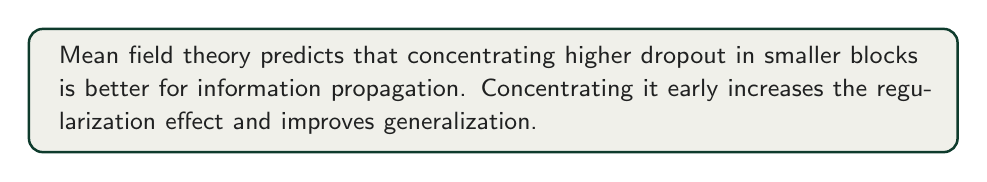
\begin{tikzpicture}
    \node[
      fill=forest!10!paper,
      fill opacity=0.45,
      draw=forest,
      line width=0.9pt,
      text opacity=1,
      text=ink,
      rounded corners=5pt,
      inner xsep=0.38cm,
      inner ysep=0.22cm,
      text width=0.91\textwidth,
      align=left
    ] {\small 
    Mean field theory predicts that concentrating higher dropout in smaller blocks is better for information propagation. Concentrating it early increases the regularization effect and improves generalization.};
  \end{tikzpicture}

  \vspace{0.35em}
  \begin{center}
  \begin{minipage}{0.91\textwidth}
  \begin{columns}[T,onlytextwidth]
    \begin{column}{0.50\textwidth}
      \centering
      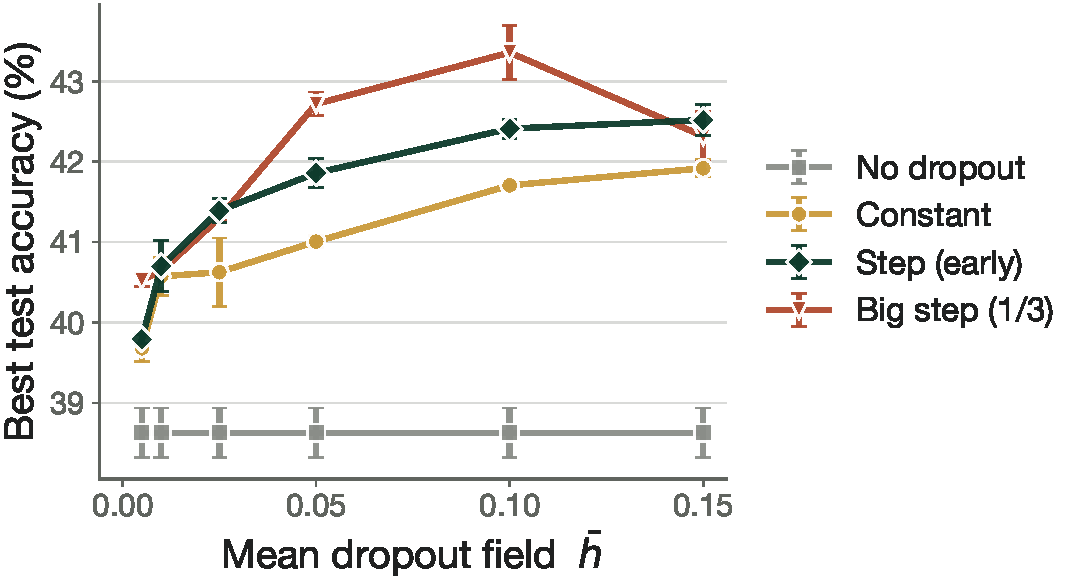
\includegraphics[height=0.44\textheight]{assets/results/h_sweep_schedule_styled.pdf}
    \end{column}

    \begin{column}{0.48\textwidth}
      \centering
      \vspace{0.0em}
      \footnotesize
      \renewcommand{\arraystretch}{1.15}
      \begin{tabular}{@{}lcc@{}}
        \toprule
        Setting & best schedule & loss reduction \\
        \midrule
        MLP overfitting    & Step (early) & \(17.9\%\) \\
        MLP budget control & Big step     & \(22.6\%\) \\
        \relu{} sweep      & Big step     & \(35.4\%\) \\
        GELU sweep         & Big step     & \(29.8\%\) \\
        ViT CIFAR-100      & Linear dec.  & \(4.2\%\)  \\
        ViT ablations      & Step (early) & \(6.3\%\)  \\
        \bottomrule
      \end{tabular}
    \end{column}
  \end{columns}
  \end{minipage}
  \end{center}
\end{frame}

% -------------------------------------------------------------------------
% Close
% -------------------------------------------------------------------------
\begin{frame}[plain]
  \vfill
  \begin{center}
    {\fontsize{26}{31}\selectfont\color{forest}\bfseries Front-load your dropout!}\\[0.5em]
    {\fontsize{15}{20}\selectfont\color{ink}%
      Higher accuracy and lower test loss, no extra cost!}

    \vspace{0.85cm}
    {\color{gold}\rule{6.5cm}{1.0pt}}

    \vspace{1.0cm}
    {\large\color{forest}\bfseries Thank you}\\[0.25em]
    {\scriptsize\color{muted}Lucas Fernandez-Sarmiento \(\cdot\) Carnegie Mellon University \(\cdot\) ICML 2026}
  \end{center}
  \vfill
\end{frame}

\end{document}
